\documentclass[10pt]{article}
\usepackage{fourier}
\usepackage{lingmacros}
\usepackage{graphicx}
\usepackage{caption}
\usepackage{subcaption}
\usepackage{amsmath}
\usepackage[margin=0.5in]{geometry}

\begin{document}

\title{Symbols, Patterns \& Signals - CW2: A Memory of Wine}
\author{Saif Anwar \& Tommy Van Aalst}
\date{}
\maketitle


\section*{Introduction}
\section*{Choosing the best features}

To choose the best features we observed all the plots of the pairwise combinations of the features and tried to find the ones which separated the data points into the three classes the best.
There are some which clearly do not work, because the data points are overlapping and there is clearly no way to separate them into their three classes.

\begin{figure}[h!]
\captionsetup[subfigure]{labelformat=empty}
\begin{subfigure}{.5\textwidth}
\centering
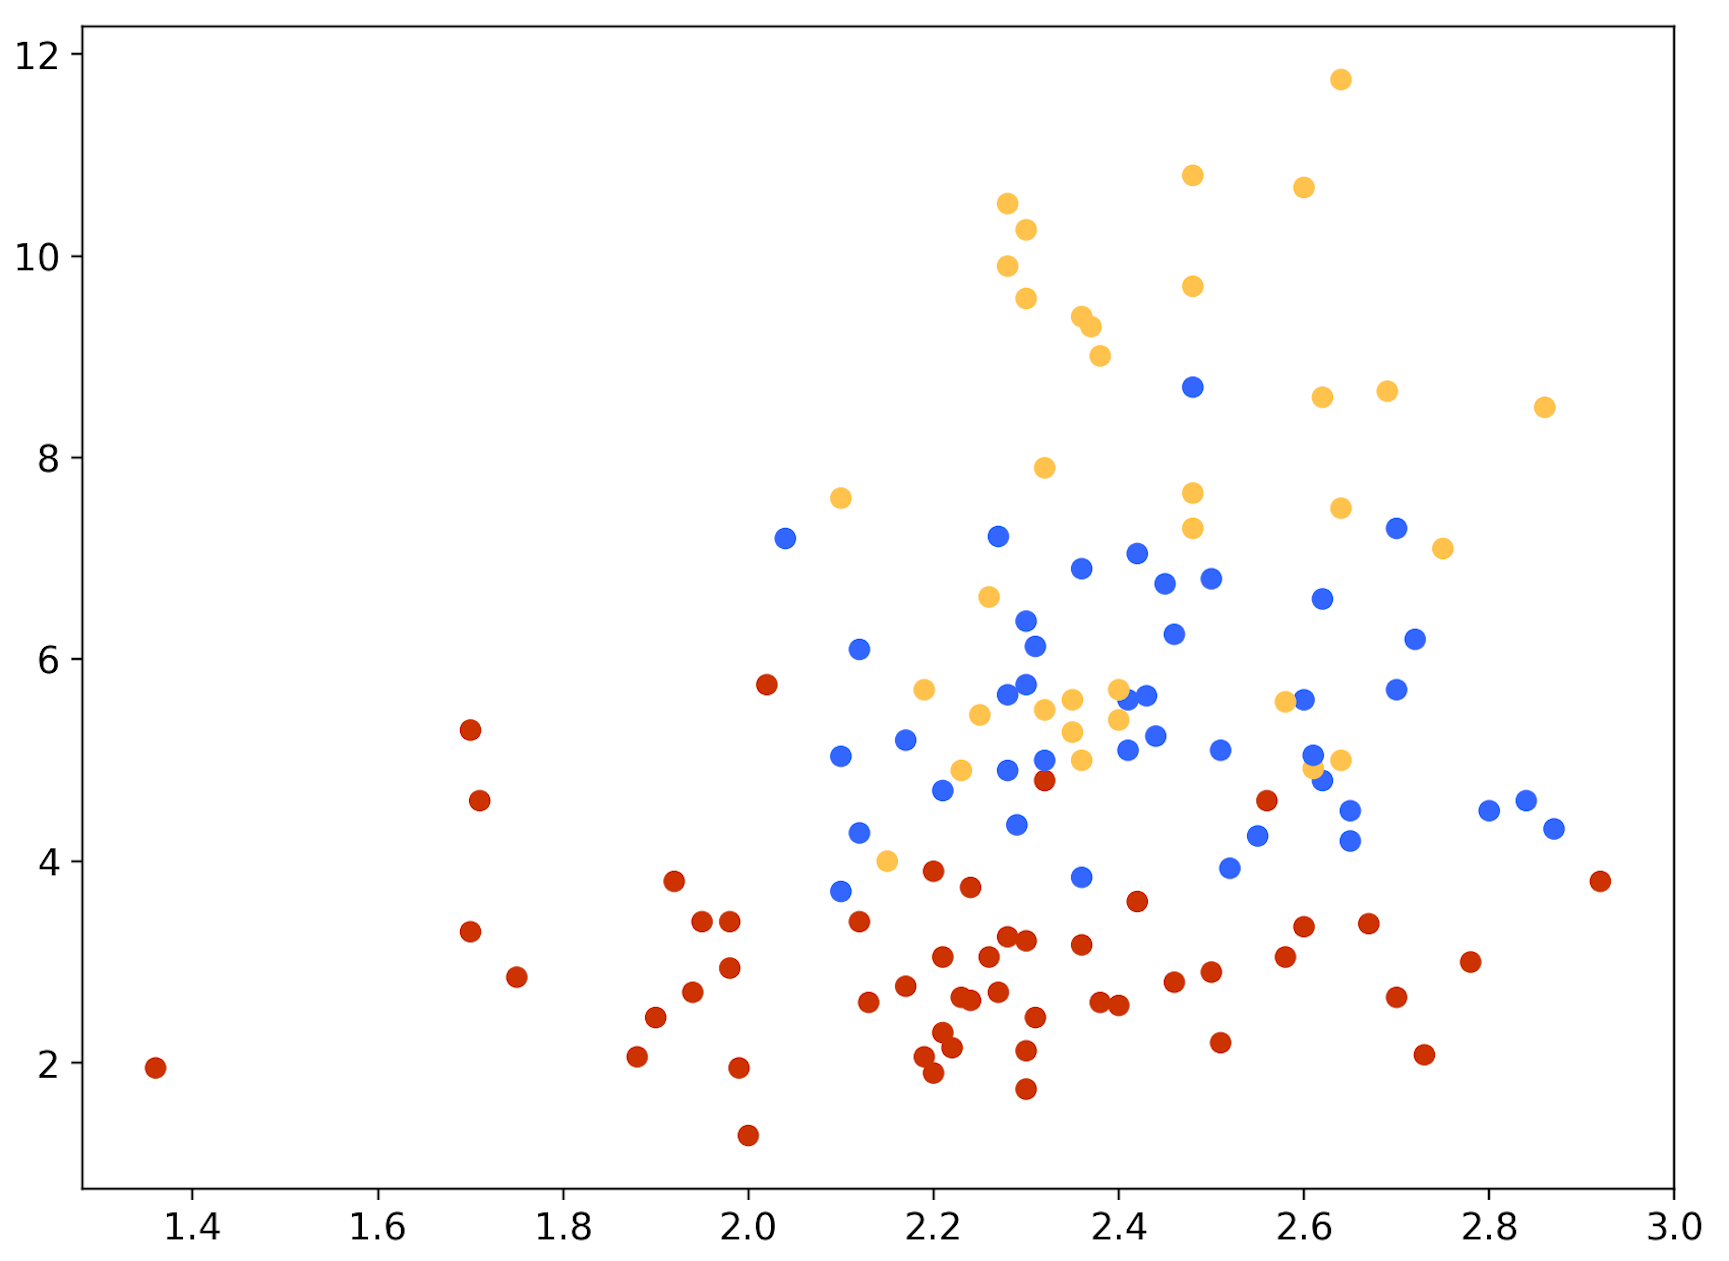
\includegraphics[height=4.2cm]{3and10.png}
\caption{Fig 1: Plot of features 3 and 10}
\end{subfigure}%
\begin{subfigure}{.5\textwidth}
\centering
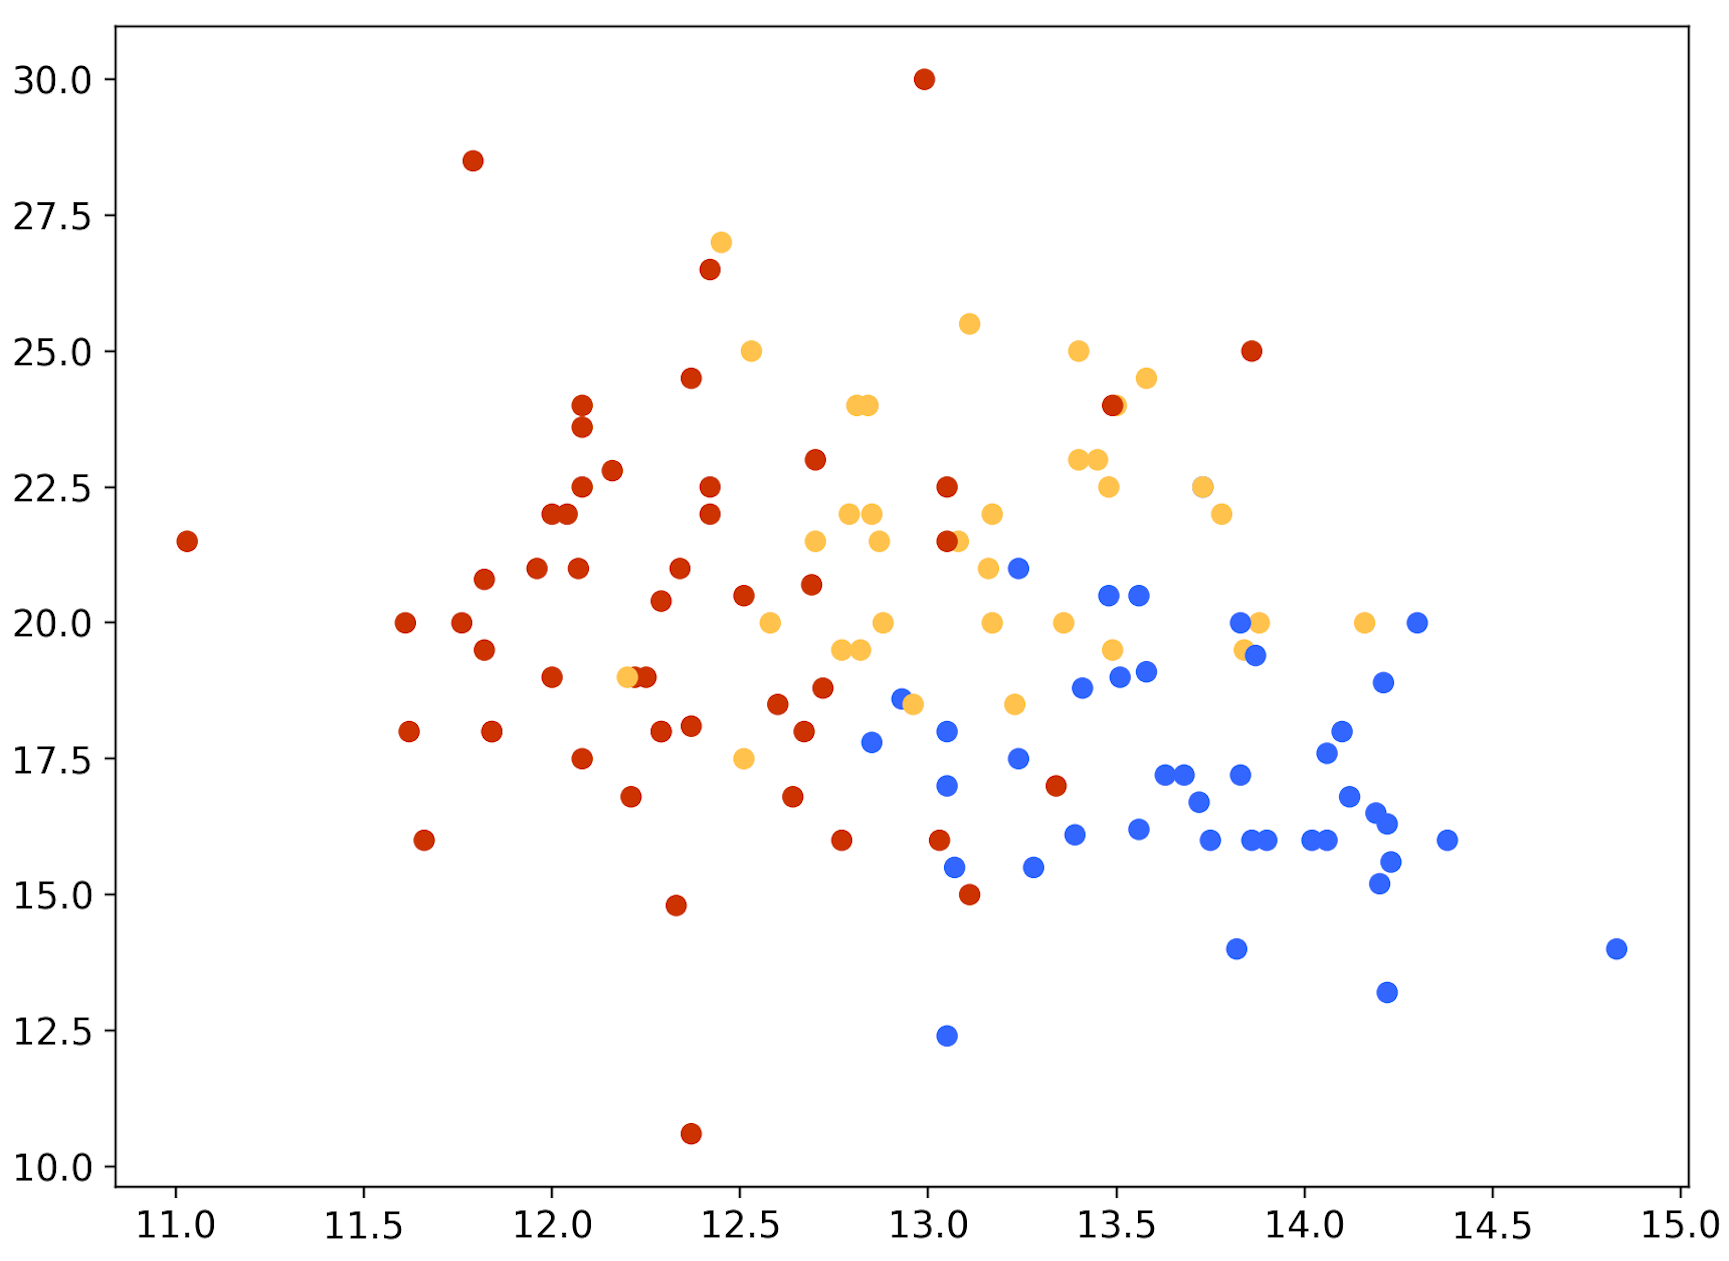
\includegraphics[height=4.2cm]{1and4.png}
\caption{Fig 2: Plot of features 1 and 4}
\end{subfigure}%
\end{figure}
\noindent
Here you can see in Fig 1 that although the red class is somewhat separable from the other two, the blue and yellow completely mix. It would be impossible to separate them in any way. In Fig 2 each class is in its own part of the plot, however in the middle they all overlap, again meaning there is no way to clearly separate the points into their three classes.\\

\noindent
There are also a quite a few which do all work well, like these ones below:

\begin{figure}[h!]
\captionsetup[subfigure]{labelformat=empty}
\begin{subfigure}{.5\textwidth}
\centering
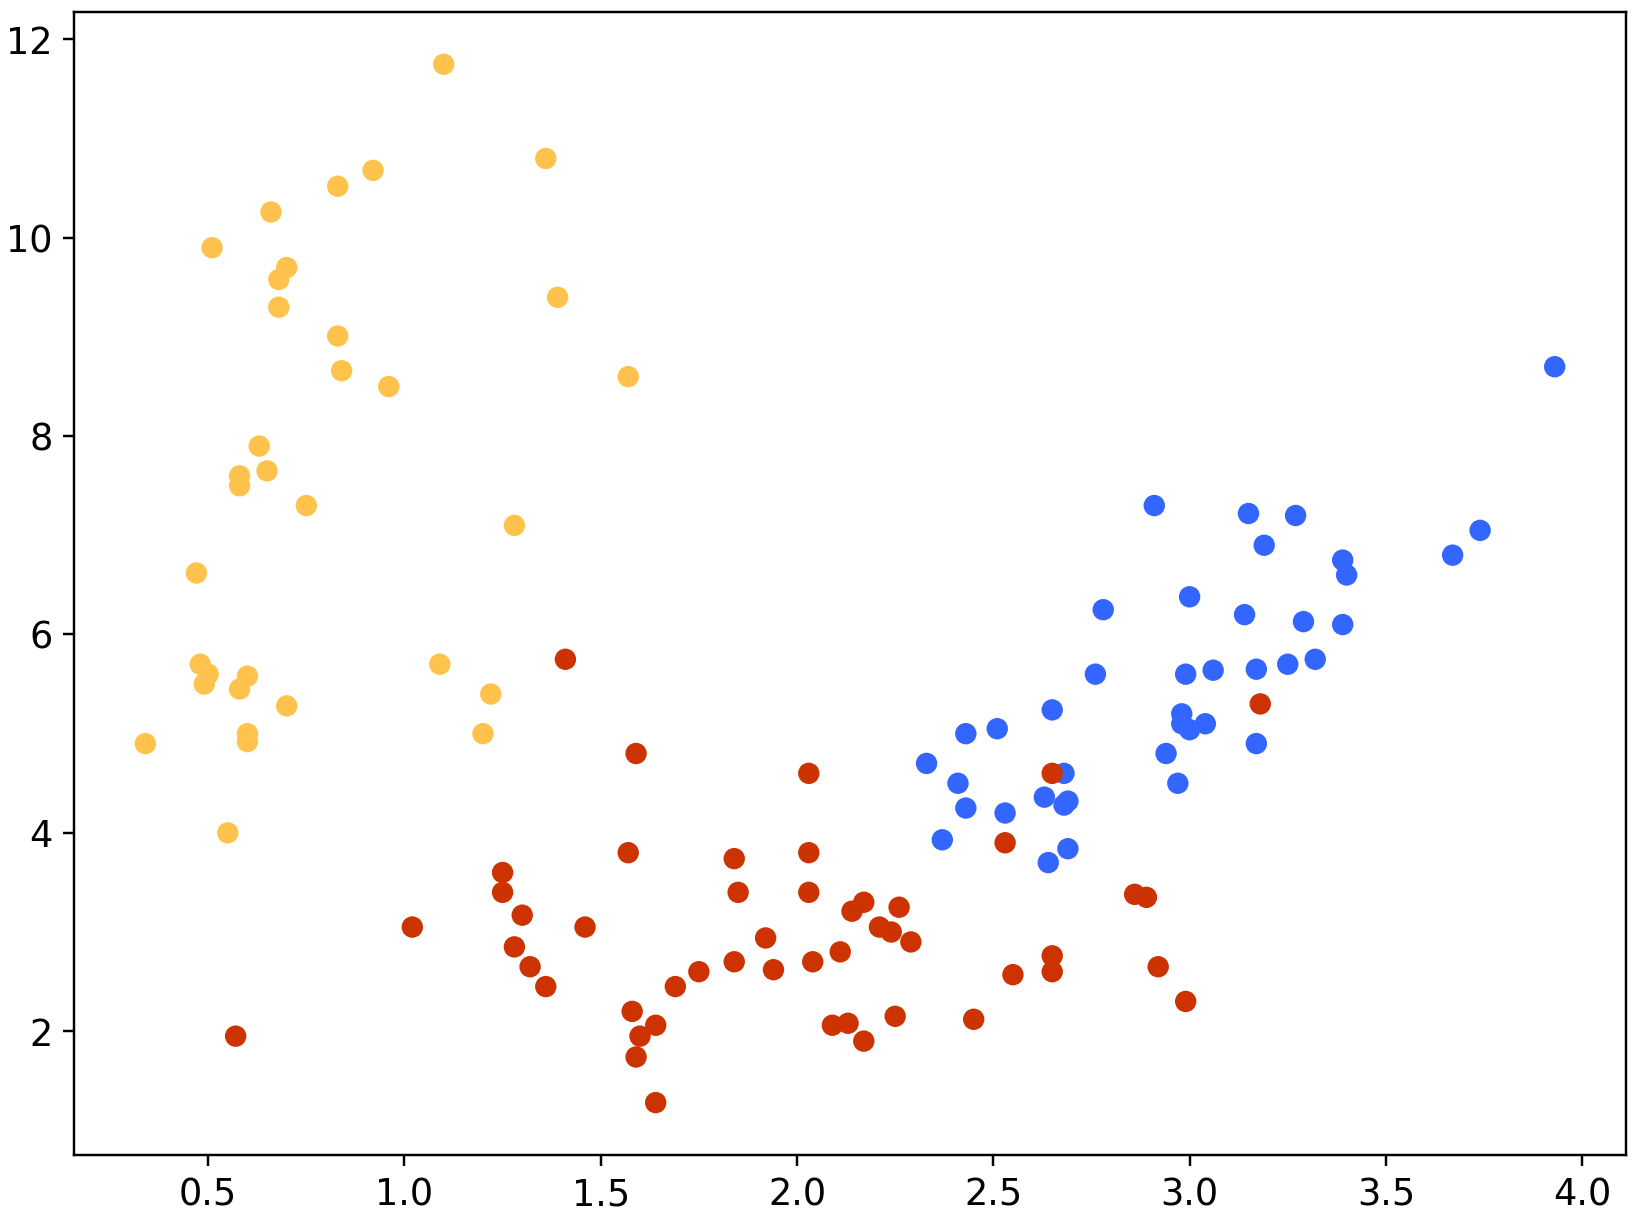
\includegraphics[height=4.2cm]{7and10.png}
\caption{Fig 3: Plot of features 7 and 10}
\end{subfigure}%
\begin{subfigure}{.5\textwidth}
\centering
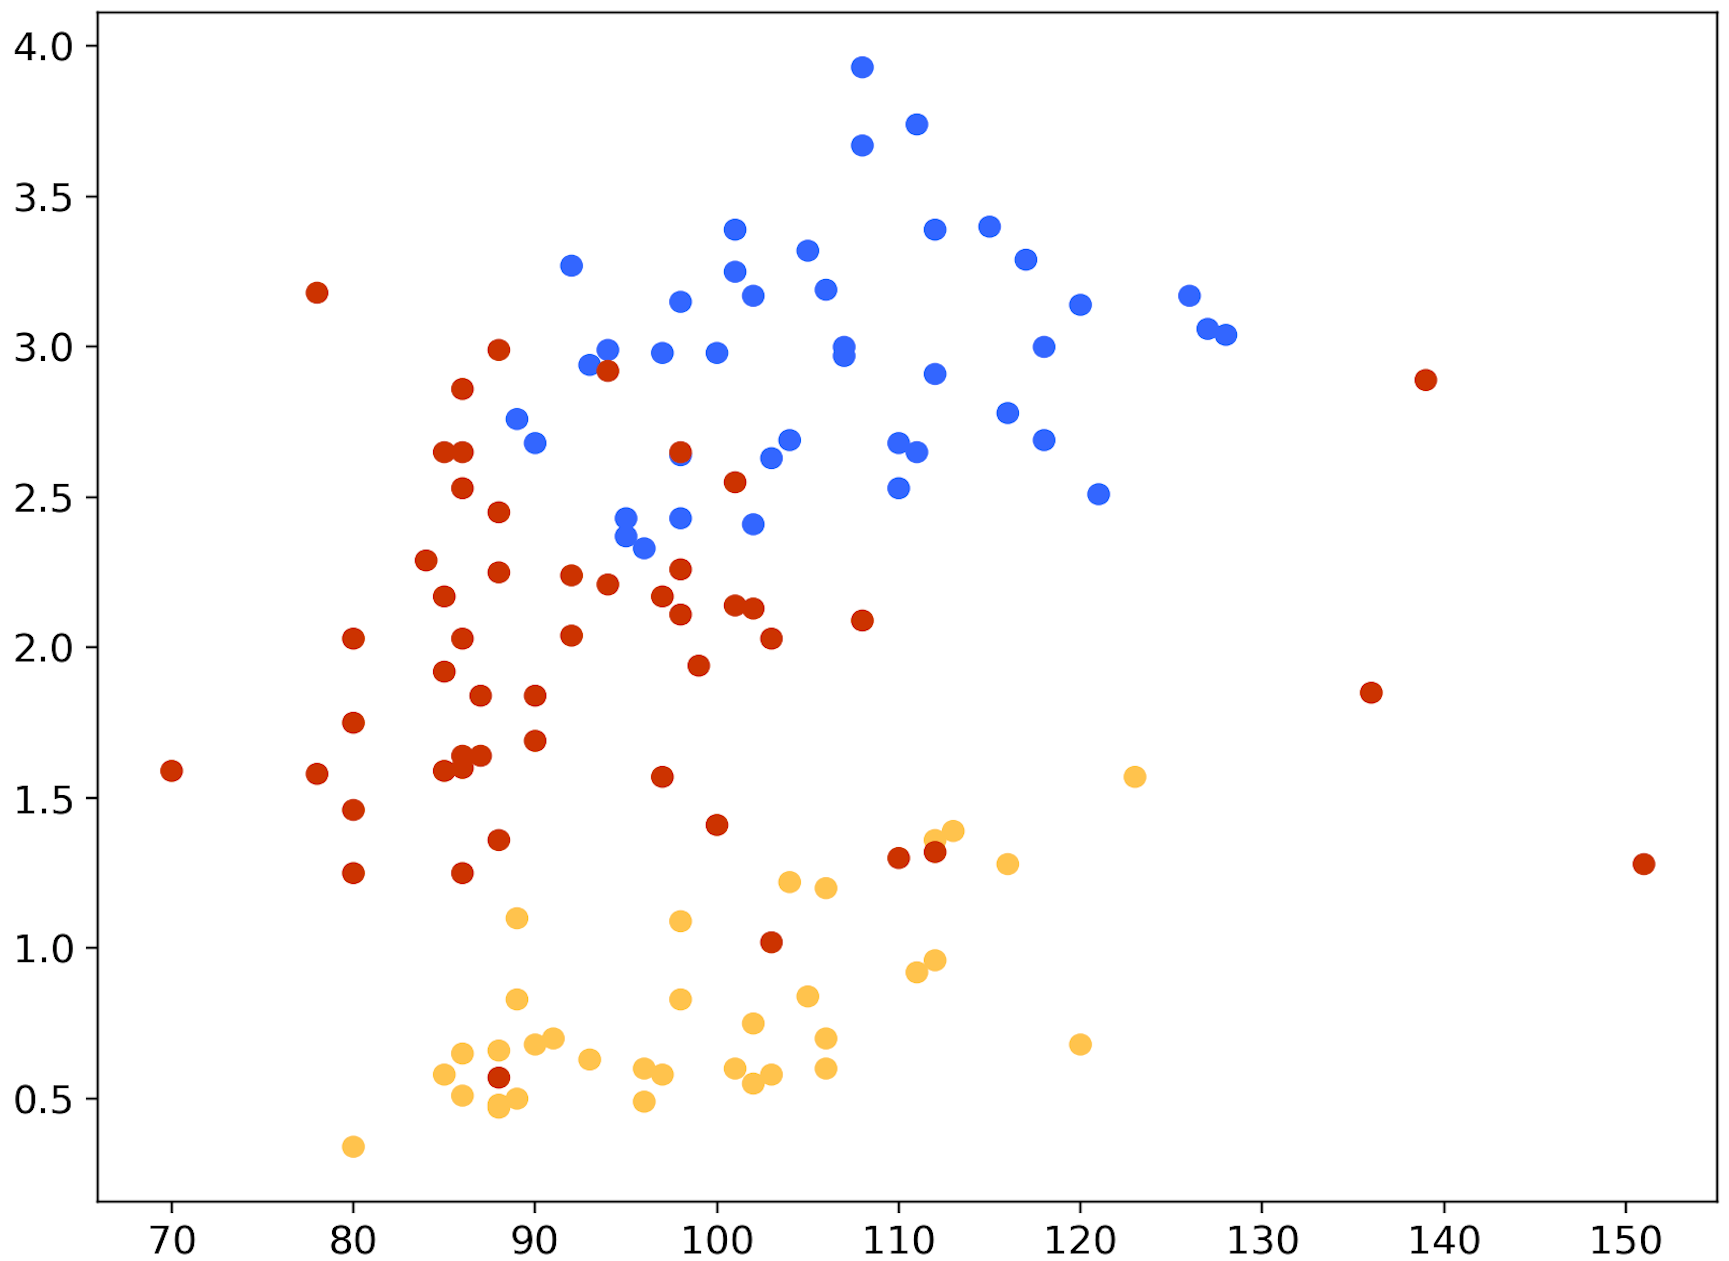
\includegraphics[height=4.2cm]{5and7.png}
\caption{Fig 4: Plot of features 5 and 7}
\end{subfigure}%
\end{figure}
\noindent
\\
\noindent
Here you can see clearly in Fig 3 that you can separate each of the classes well. There is some slight overlap on the edges but not much. Also, each class only has a boundary to one other class. All three classes don’t overlap together in the middle so the boundary data could be only one of two classes, not one of three, therefore resulting in more accurate predictions. Fig 4 is quite good however there is a little bit of overlap between the blue and red classes and the red class has some outliers spread out. We concluded to choose features 7 and 10.\\

\noindent
We also ran a script to calculate the accuracies of each pairwise combination. We found that the features we chose gave relatively good accuracy in each of our classifiers.

\section*{K-Nearest Neighbours}

We implemented the K-Nearest Neighbours (knn) algorithm using functions to represent the steps. The first step is to calculate the Euclidean Distance between the wine in question from the wine\_test set and every wine from the wine\_train set. For a two-dimensional knn this will only be for the two selected features using the following formula:
$$d(x,y) = \sqrt{\sum_{n=1}^{k} (x_i - y_i)}$$
\\
\noindent
From all of these distances we can now find the k smallest distances to get the nearest neighbours when the test wine is plotted onto the scatter of the train sets selected features.\\

\noindent
Now we have to assign a class to each of the neighbours by reading the wine\_train\_labels file to get an idea of what classes are closest to our test wine graphically. From this we can assume and assign a class to our test wine. Depending on the selected number of nearest neighbours, k, we may or may not have a modal class amongst our neighbours. If k=1 then we have an obvious mode of the single class and our test wine can be assumed to be of this class. Any k higher than this invites the possibility for multiple mode classes in the nearest neighbours. In this situation we recalculate the modal classes for k-1 neighbours which eliminates the furthest neighbour. This is repeated until we successfully find a mode which is then assigned as our test wines class.\\

\noindent
We can repeat this process for each of the wines in the wine\_test set and create our list of predictions for the test set. By comparing our predictions with the provided wine\_test\_labels, we can calculate an accuracy for our algorithm using the following formula:
$$Accuracy = \frac{\text{Number of Correctly Predicted Wines}}{\text{Total Number of Wines}}$$
\begin{figure}[h!]
\captionsetup[subfigure]{labelformat=empty}
\begin{subfigure}{\textwidth}
\captionsetup[figure]{labelformat=empty}
\centering
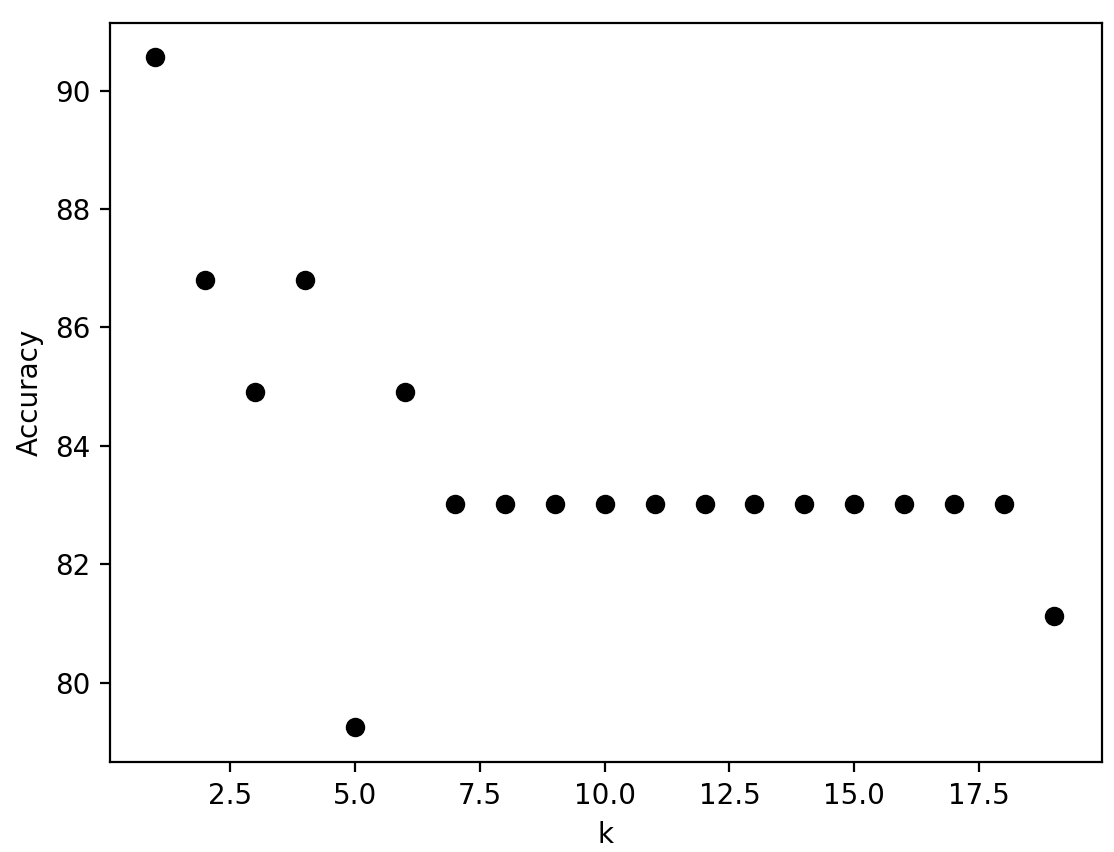
\includegraphics[height=4.2cm]{accuracies.png}
\caption{Fig 5: Plot of k and accuracies}
\end{subfigure}%
\end{figure}
\\
\noindent
Fig 5 shows the effect increasing the number of neighbours, k, has on the accuracy of the classifier whilst the selected features remain the same. As can be observed from the figure, features (7 and 10) would get a reasonably high accuracy of 90.57\% at k=1. As the number of nearest neighbours is increased, we observe a lower accuracy until k=5 where after that it begins to increase again. This would be due to an increase in incorrect classification based on closest neighbours. The figure shows the accuracies for k in the range 0-20. It can also be seen that at a certain value of k, the accuracy plateaus. This can be assumed to be due to the wine in question being in a region where the modal class is the mode by a significant number.\\

\noindent
Here are the confusion matrices for each of the values of $k \in (1,2,3,4,5,6,7)$

$$
k=1
\begin{bmatrix} 
1 & 0 & 0\\
0.19 & 0.81 & 0\\
0 & 0.07 & 0.93
\end{bmatrix}
\quad
k=2
\begin{bmatrix} 
1 & 0 & 0\\
0.24 & 0.76 & 0\\
0 & 0.14 & 0.86
\end{bmatrix}
\quad
k=3
\begin{bmatrix} 
0.89 & 0.11 & 0\\
0.19 & 0.81 & 0\\
0 & 0.14 & 0.86
\end{bmatrix}
\quad
k=4
\begin{bmatrix} 
1 & 0 & 0\\
0.24 & 0.76 & 0\\
0 & 0.14 & 0.86
\end{bmatrix}
$$
$$
k=5
\begin{bmatrix} 
0.78 & 0.22 & 0\\
0.24 & 0.76 & 0\\
0 & 0.14 & 0.86
\end{bmatrix}
\quad
k=6
\begin{bmatrix} 
0.94 & 0.06 & 0\\
0.24 & 0.76 & 0\\
0 & 0.14 & 0.86
\end{bmatrix}
\quad
k=5
\begin{bmatrix} 
0.89 & 0.11 & 0\\
0.24 & 0.76 & 0\\
0 & 0.14 & 0.86
\end{bmatrix}
\quad
$$
\\
\noindent
It can be observed that there are no wrong predictions between 1 and 3 (1 being classed as three and vice versa). This was expected as there is not an approximate boundary, in the scatter plot of the features, that is shared by both classes 1 (Blue) and 3 (Yellow). Also we can see that there is the most discrepancy between the classification of wines that are actually class 2 (Red) but being classed as 1. This was to be expected from the visible overlap between the two classes in the plot of the features (Fig 3).

\section*{Alternate Classifier - Na\"ive Bayes Classifier}
-We implemented Naive Bayes Classifier as our alternative classifier. With the same features used for K-NN, (7 and 10), we got an accuracy of 62.3\%. This is a fair bit worse than K-NN with one neighbour which has an accuracy of 90.6\%. This could be due to the fact that K-NN is a discriminative classifier, whereas Naive Bayes is a generative classifier, therefore K-NN looks at just classifying the given data with a boundary between the two datasets by only looking at the data but Naive Bayes tries to assume where to classify the data based on how the previous data was generated. Most of the time discriminative classifiers are better than generative ones and our data supports this claim.\\

\noindent
K-NN has running time O(n) whereas Naive Bayes is almost O(1) time. This would mean in a larger dataset, K-NN would be less efficient, but since our data set is fairly small, there is no need to worry about run time and we can choose the best classifier.
With K-NN the decision boundaries can take on any form, since its non-parametric, which when we have good feature selection this is means accuracy can be very high, whereas Bayes does not do this.\\

\noindent
Because of the fact that K-NN optimises locally by viewing an area around the given datapoint, outliers would seriously affect the accuracy since they could be in a cluster of different data points. When there are more outliers in the data, Naive Bayes would be a better choice of classifier since it doesn't have this problem. However, we have chosen good features with very few outliers and so in this case, with these features, K-NN would be preferable and the results support this.
\\
\section*{K-Nearest Neighbours with three features}

Constructing the KNN Classifier with 3 features adds a new dimension to calculating the Euclidean Distance between the points. It incorporates all the possible combinations of the three features. For example, we selected features 1,2 and 7; proceeded to plot them on a 3-dimensional axis to observe the boundaries between the classes. Observing the 3d scatter plot perpendicular to each of the axis will give you the 2d plot of the other two features. Doing this in turn will give you an idea of the relationship between each of the features individually. \\

\noindent
Here are some plots of features 1,2 and 7 in 3d space from each axis:

\begin{figure}[h!]
\captionsetup[subfigure]{labelformat=empty}
\begin{subfigure}{.33\textwidth}
\centering
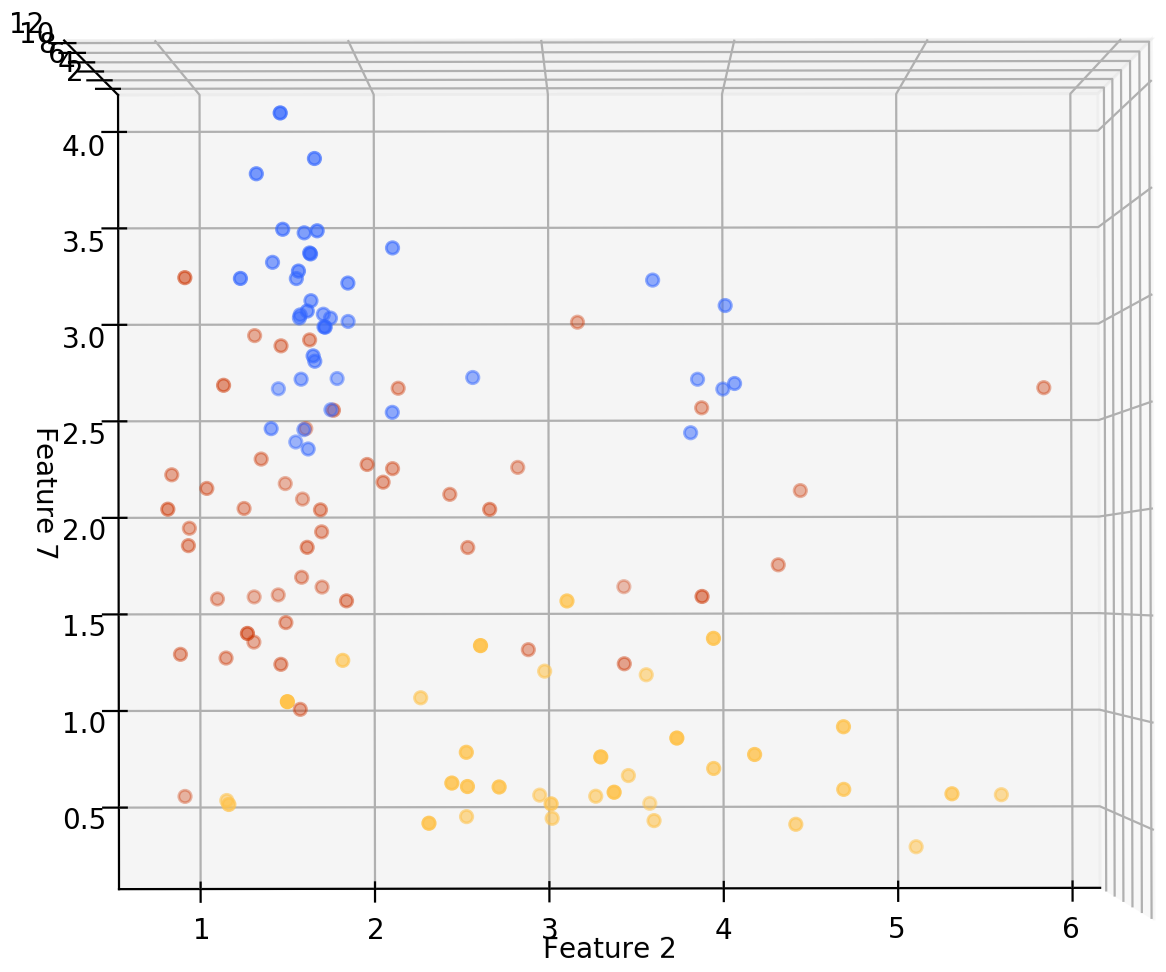
\includegraphics[height=4.2cm]{3d2x7.png}
\caption{Fig 5: Plot of features 2 and 7 in 3d space}
\end{subfigure}%
\begin{subfigure}{.33\textwidth}
\centering
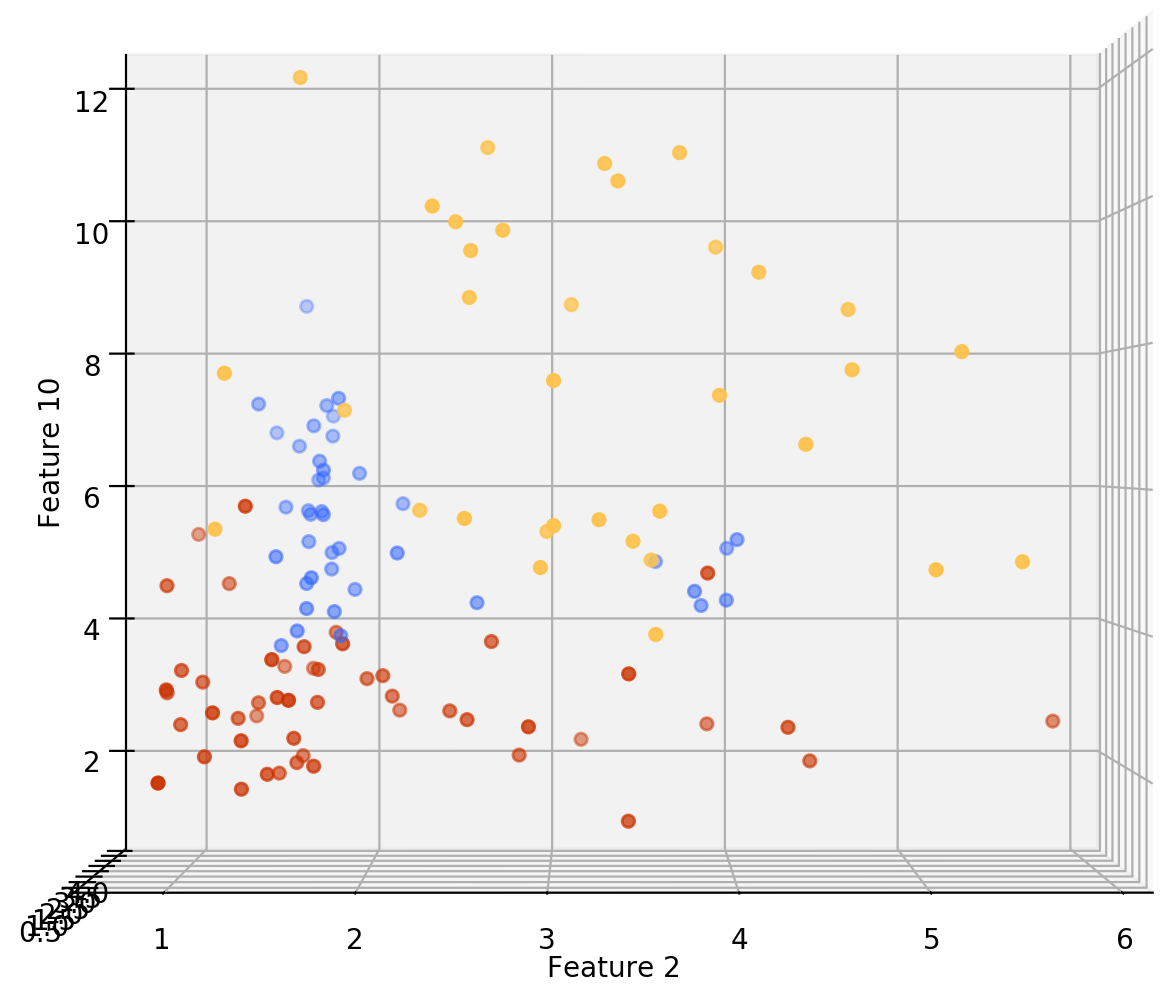
\includegraphics[height=4.2cm]{3d2x10.png}
\caption{Fig 6: Plot of features 2 and 10 in 3d space}
\end{subfigure}%
\begin{subfigure}{.33\textwidth}
\centering
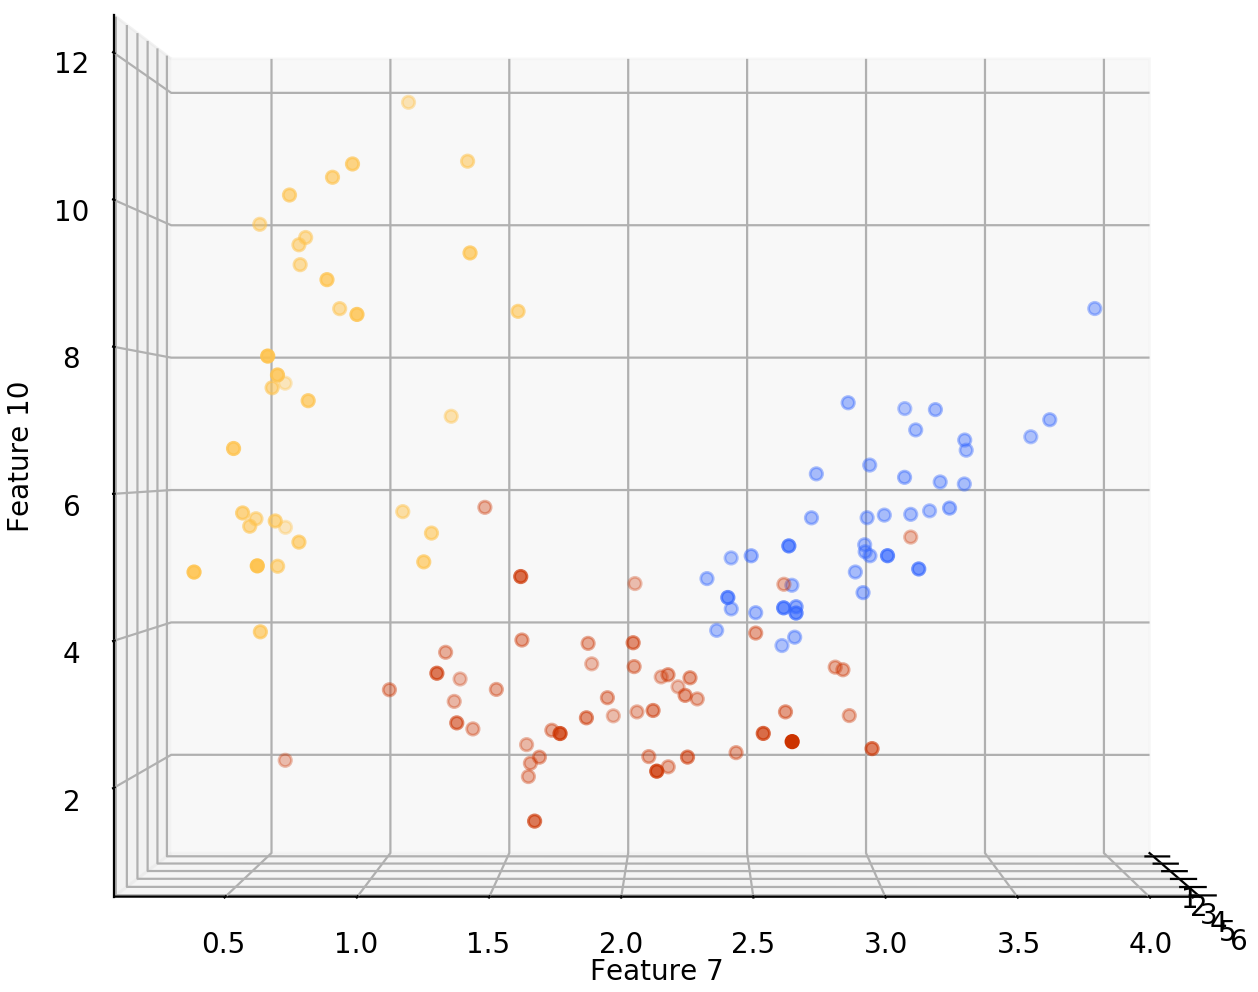
\includegraphics[height=4.2cm]{3d7x10.png}
\caption{Fig 7: Plot of features 7 and 10 in 3d space}
\end{subfigure}%
\end{figure}

\noindent
Using three features can either be beneficial by picking features that compliment each other in their individual plots against the other features, or can in fact make the classifier worse overall due to a single pair of the combinations not showing a strong distinctive relationship between the classes. To select our 3 features, we kept our 2 features from our original KNN classifier so we could see what difference a single new dimension would make without changing our other features. We used a script to calculate the accuracy from each selection and we deemed feature 2 to be a fitting addition to the KNN classifier.  As can be seen in the figures above, each of the pairwise combinations of features show reasonable boundaries between each of the classes confirming that (2,7,10) is a suitable set of features to use for our 3d KNN classifier. \\

\noindent
We can compare the accuracy between using 3 features and using 2 features by comparing the confusion matrices for $k \in (1,2,3,4,5,6,7)$:

$$
k=1
\begin{bmatrix} 
1 & 0 & 0\\
0.1 & 0.9 & 0\\
0 & 0.07 & 0.93
\end{bmatrix}
\quad
k=2
\begin{bmatrix} 
1 & 0 & 0\\
0.24 & 0.76 & 0\\
0 & 0.07 & 0.93
\end{bmatrix}
\quad
k=3
\begin{bmatrix} 
0.94 & 0.06 & 0\\
0.19 & 0.81 & 0\\
0 & 0.07 & 0.93
\end{bmatrix}
\quad
k=4
\begin{bmatrix} 
0.94 & 0.06 & 0\\
0.24 & 0.76 & 0\\
0 & 0.07 & 0.93
\end{bmatrix}
$$
$$
k=5
\begin{bmatrix} 
0.89 & 0.11 & 0\\
0.19 & 0.81 & 0\\
0 & 0.07 & 0.93
\end{bmatrix}
\quad
k=6
\begin{bmatrix} 
0.89 & 0.11 & 0\\
0.24 & 0.76 & 0\\
0 & 0.07 & 0.93
\end{bmatrix}
\quad
k=7
\begin{bmatrix} 
0.89 & 0.11 & 0\\
0.24 & 0.76 & 0\\
0 & 0.07 & 0.93
\end{bmatrix}
\quad
$$
\noindent
\\
\noindent
From the confusion matrices of KNN3d we can deduce that the accuracies are generally better than the KNN with 2 features. However  The plot of features 2 \& 10 shows multiple crossovers the classes and doesn’t show distinct boundaries. This would negatively affect our classifier when taking more neighbours into account as shown by the trend where accuracy decreases as k increases. This can be seen to possibly be due to the pairwise combination of features 2 \& 7 where there is significant crossover between class 1 (Blue) and class 2 (Red).

\section*{K-Nearest Neighbours Using Principle Component Analysis (PCA)}
KNN is a technique that is generally likely to overfit the data which is why there is a need to optimise the value of k and carefully select features which represent the train data and future data in a fair way. One way to reduce the effect of overfitting is to increase the size of the training data but with KNN being $\mathcal{O}(n)$ a Principal Component Analysis (PCA) is a method to reduce the dimensionality of the data. It extracts the most useful parts of the data whilst aiming to maintain the same level of accuracy within the classifier. Using the PCA implementation from the Scipy library, we reduced our training data.\\

\noindent
The following is a scatter plot of the PCA-reduced data and the original scatter plot of the features we selected:


\noindent

\begin{figure}[h!]
\captionsetup[subfigure]{labelformat=empty}
\begin{subfigure}{.5\textwidth}
\centering
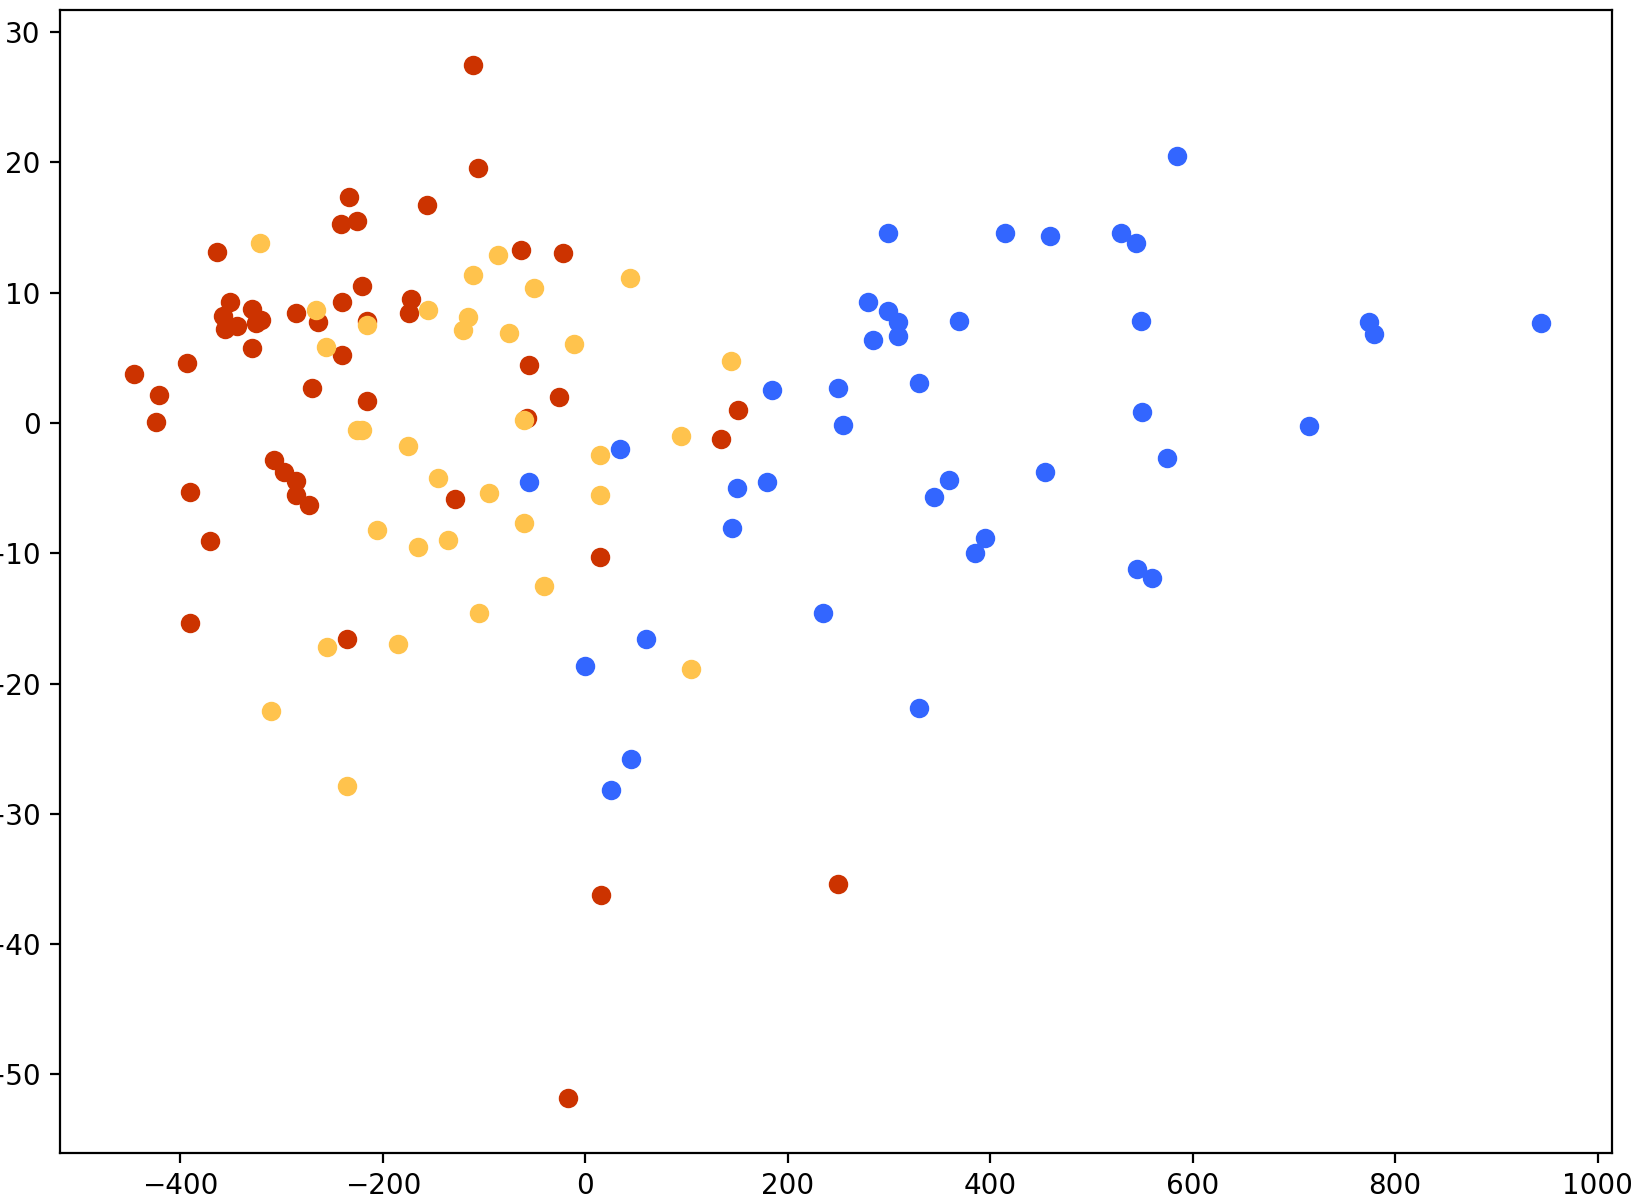
\includegraphics[height=4.2cm]{pca.png}
\caption{Fig 8: Plot of PCA-reduced train\_set}
\end{subfigure}%
\begin{subfigure}{.5\textwidth}
\centering
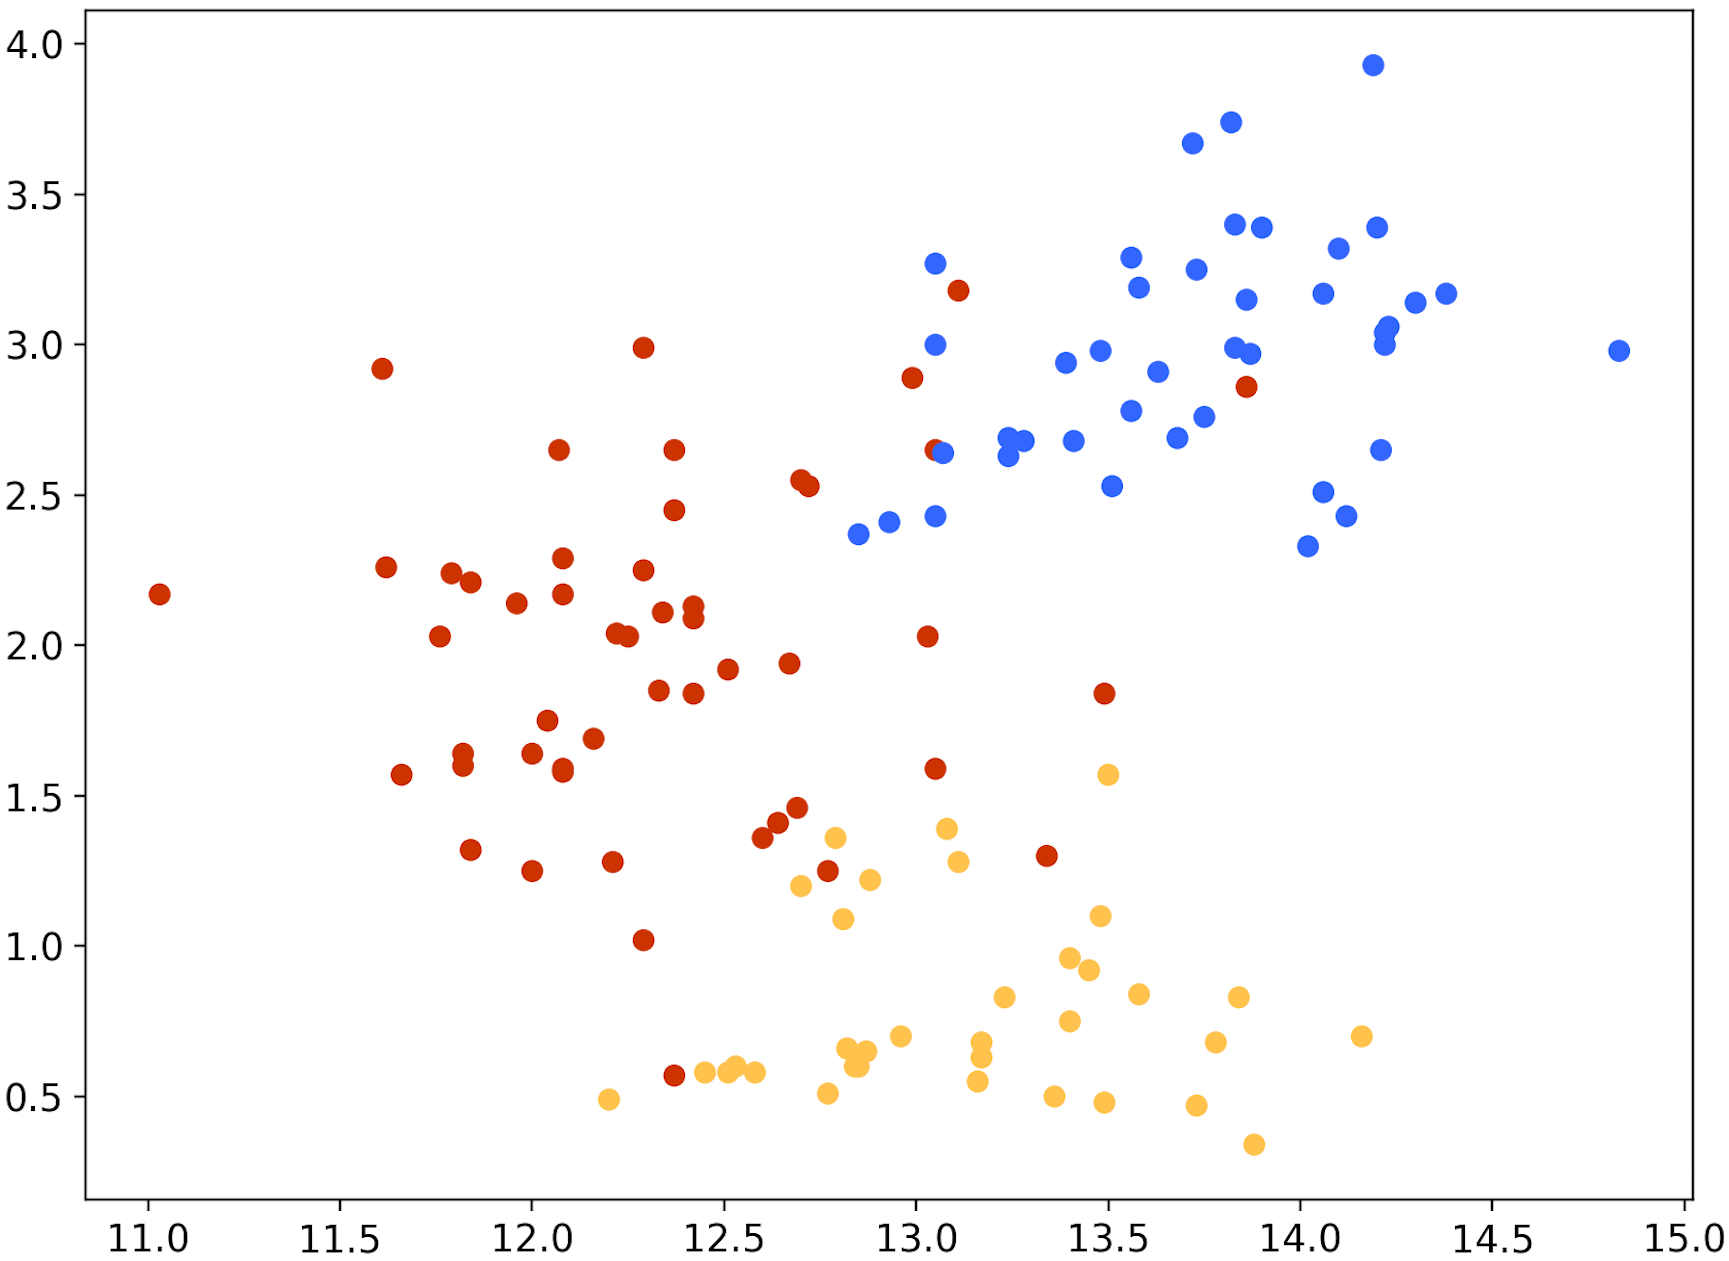
\includegraphics[height=4.2cm]{1and7.png}
\caption{Fig 9: Plot of features 1 and 7}
\end{subfigure}%
\end{figure}
\noindent

\end{document}  























